\documentclass[letterpaper,12pt,fleqn]{article}
\usepackage{matharticle}
\pagestyle{empty}
\newcommand{\nnorm}[2]{\left\|#1\right\|_{#2}}
\newcommand{\norm}[1]{\nnorm{#1}{}}
\newcommand{\inorm}[1]{\nnorm{#1}{\infty}}
\newcommand{\lonorm}[1]{\nnorm{#1}{L_1}}
\newcommand{\vv}{\vec{v}}
\newcommand{\vx}{\vec{x}}
\newcommand{\vy}{\vec{y}}
\newcommand{\vo}{\vec{0}}
\newcommand{\cf}{\mathcal{C}}
\newcommand{\F}{\mathbb{F}}
\renewcommand{\a}{\alpha}
\renewcommand{\b}{\beta}
\renewcommand{\l}{\lambda}
\newcommand{\e}{\epsilon}
\renewcommand{\d}{\delta}
\begin{document}
\section*{Equivalent Norms}

\begin{definition}[Equivalence]
  Let $E$ be a normed vector space and let $\nnorm{\cdot}{1}$ and
  $\nnorm{\cdot}{2}$ be two norms on $E$. To say that $\nnorm{\cdot}{1}$ and
  $\nnorm{\cdot}{2}$ are \emph{equivalent} on $E$ means
  $\forall\,(\vx_n),x\in E$:
  \[\nnorm{x_n-x}{1}\to0\iff\nnorm{x_n-x}{2}\to0\]
\end{definition}

\begin{example}
  Let $E=\cf[0,1]$:

  \qquad$\inorm{\cdot}$ is not equivalent to $\lonorm{\cdot}$.

  Consider $f_n(t)=t^n$:

  \begin{minipage}{2.5in}
    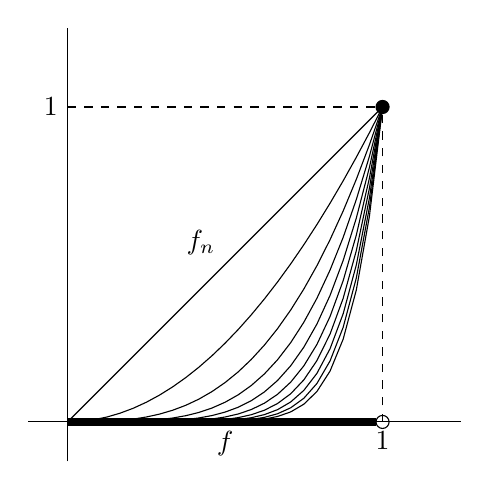
\begin{tikzpicture}
      \draw (-0.5,0) -- (5,0);
      \draw (0,-0.5) -- (0,5);
      \node [below] at (4,0) {$1$};
      \node [left] at (0,4) {$1$};
      \draw [dashed] (0,4) -- (4,4);
      \draw [dashed] (4,0) -- (4,4);
      \draw [domain=0:4] plot ({\x},{\x});
      \draw [domain=0:4] plot ({\x},{4*(\x/4)^2});
      \draw [domain=0:4] plot ({\x},{4*(\x/4)^3});
      \draw [domain=0:4] plot ({\x},{4*(\x/4)^4});
      \draw [domain=0:4] plot ({\x},{4*(\x/4)^5});
      \draw [domain=0:4] plot ({\x},{4*(\x/4)^6});
      \draw [domain=0:4] plot ({\x},{4*(\x/4)^7});
      \draw [domain=0:4] plot ({\x},{4*(\x/4)^8});
      \draw [domain=0:4] plot ({\x},{4*(\x/4)^9});
      \draw [domain=0:4] plot ({\x},{4*(\x/4)^10});
      \node [draw, circle, scale=0.5] (a) at (4,0) {};
      \node [draw, fill, circle, scale=0.5] (b) at (4,4) {};
      \draw [line width=1mm] (0,0) to (a);
      \node [above left] at (2,2) {$f_n$};
      \node [below] at (2,0) {$f$};
    \end{tikzpicture}
  \end{minipage}
  \begin{minipage}{3in}
    \[f_n(t)\to f(t)=\begin{cases}
    1, & 0\le t<1 \\
    0, & t=1
    \end{cases}\]
  \end{minipage}

  Comparing the two norms:
  \[\lonorm{f_n-0}=\lonorm{f_n}=\int_0^1t^ndt=\left.\frac{t^{n+1}}{n+1}
  \right|_0^1=\frac{1}{n+1}\to 0\]
  But:
  \[\inorm{f_n-0}=\inorm{f_n}=\max_{0\le t\le1}\{t^n\}=1\ne0\]
\end{example}

\begin{theorem}
  Let $E$ be a normed vector space and let $\nnorm{\cdot}{1}$ and
  $\nnorm{\cdot}{2}$ be two norms on $E$. $\nnorm{\cdot}{1}$ and
  $\nnorm{\cdot}{2}$ are equivalent iff $\exists\,\a,\b>0$ such that
  $\forall\,\vx\in E$:
  \[\a\nnorm{\vx}{1}\le\nnorm{\vx}{2}\le\b\nnorm{\vx}{1}\]
\end{theorem}

\begin{theproof}
  \listbreak
  \begin{description}
  \item $\implies$ Assume $\nnorm{\cdot}{1}$ and $\nnorm{\cdot}{2}$ are
    equivalent.

    $\forall\,(\vy_n),\vy\in E, \nnorm{\vy_n-\vy}{1}\to0\iff
    \nnorm{\vy_n-\vy}{2}\to0$ \\
    Let $\vy=\vo$ \\
    $\forall\,(\vy_n)\in E, \nnorm{\vy_n-\vo}{1}\to0\iff
    \nnorm{\vy_n-\vo}{2}\to0$ \\
    $\forall\,(\vy_n)\in E, \nnorm{\vy_n}{1}\to0\iff\nnorm{\vy_n}{2}\to0$

    ABC: $\forall\,\a,\b>0,\exists\,\vx\in E,
    \a\nnorm{\vx}{1}>\nnorm{\vx}{2}$ or $\nnorm{\vx}{2}>\b\nnorm{\vx}{1}$.

    Let $\a=\frac{1}{n}$ and $\b=n$. \\
    $\exists\,\vx_n\in E$ such that $\frac{1}{n}\nnorm{\vx_n}{1}>
    \nnorm{\vx_n}{2}$ (and so $\nnorm{\vx_n}{1}>n\nnorm{\vx_n}{2}$) or
    $\nnorm{\vx_n}{2}>n\nnorm{\vx_n}{1}$.

    \begin{description}
    \item Case 1: $\nnorm{\vx_n}{1}>n\nnorm{\vx_n}{2}$

      Let $\vy_n=\frac{1}{\sqrt{n}}\frac{\vx_n}{\nnorm{\vx_n}{2}}$:
      \[\nnorm{\vy_n}{2}=
      \nnorm{\frac{1}{\sqrt{n}}\frac{\vx_n}{\nnorm{\vx_n}{2}}}{2}=
      \frac{1}{\sqrt{n}}\frac{\nnorm{\vx_n}{2}}{\nnorm{\vx_n}{2}}=
      \frac{1}{\sqrt{n}}\to0\]
      But:
      \[\nnorm{\vy_n}{1}=
      \nnorm{\frac{1}{\sqrt{n}}\frac{\vx_n}{\nnorm{\vx_n}{2}}}{1}=
      \frac{1}{\sqrt{n}}\frac{\nnorm{\vx_n}{1}}{\nnorm{\vx_n}{2}}>
      \frac{1}{\sqrt{n}}\frac{n\nnorm{\vx_n}{2}}{\nnorm{\vx_n}{2}}=
      \sqrt{n}\to\infty\]
      So $\nnorm{\vy_n}{2}\to0$ but $\nnorm{\vy_n}{1}\to\infty$.
    
      CONTRADICTION!
      
    \item Case 2: $\nnorm{\vx_n}{2}>n\nnorm{\vx_n}{1}$

      Let $\vy_n=\frac{1}{\sqrt{n}}\frac{\vx_n}{\nnorm{\vx_n}{1}}$:
      \[\nnorm{\vy_n}{1}=
      \nnorm{\frac{1}{\sqrt{n}}\frac{\vx_n}{\nnorm{\vx_n}{1}}}{1}=
      \frac{1}{\sqrt{n}}\frac{\nnorm{\vx_n}{1}}{\nnorm{\vx_n}{1}}=
      \frac{1}{\sqrt{n}}\to0\]
      But:
      \[\nnorm{\vy_n}{2}=
      \nnorm{\frac{1}{\sqrt{n}}\frac{\vx_n}{\nnorm{\vx_n}{1}}}{2}=
      \frac{1}{\sqrt{n}}\frac{\nnorm{\vx_n}{2}}{\nnorm{\vx_n}{1}}>
      \frac{1}{\sqrt{n}}\frac{n\nnorm{\vx_n}{1}}{\nnorm{\vx_n}{1}}=
      \sqrt{n}\to\infty\]
      So $\nnorm{\vy_n}{1}\to0$ but $\nnorm{\vy_n}{2}\to\infty$.
    
      CONTRADICTION!
    \end{description}

    $\therefore\exists\,\a,\b>0,\forall\,\vx\in E,
    \a\nnorm{\vx}{1}\le\nnorm{\vx}{2}\le\b\nnorm{\vx}{1}$

    \item $\impliedby$ Assume $\exists\,\a,\b>0$ such that $\forall\,\vx\in E,
      \a\nnorm{\vx}{1}\le\nnorm{\vx}{2}\le\b\nnorm{\vx}{1}$

      Assume $(\vx_n),\vx\in E$. \\
      Assume $\a,\b>0$. \\
      $\a\nnorm{\vx_n-\vx}{1}\le\nnorm{\vx_n-\vx}{2}\le\b\nnorm{\vx_n-\vx}{1}$
      
      \begin{description}
      \item $\implies$ Assume $\nnorm{\vx_n-\vx}{1}\to0$

        $\a\nnorm{\vx_n-\vx}{1}\to0$ \\
        $\b\nnorm{\vx_n-\vx}{1}\to0$

        Therefore, by the squeeze theorem, $\nnorm{\vx_n-\vx}{2}\to0$.
        
      \item $\impliedby$ Assume $\nnorm{\vx_n-\vx}{1}\not\to0$

        $\a\nnorm{\vx_n-\vx}{1}\to x>0$ \\
        So $\nnorm{\vx_n-\vx}{2}\to y\ge x>0$

        Therefore, $\nnorm{\vx_n-\vx}{2}\not\to0$.
      \end{description}

      Therefore, $\nnorm{\cdot}{1}$ is equivalent to $\nnorm{\cdot}{1}$.
  \end{description}
\end{theproof}

\begin{theorem}
  Let $E$ be a normed space and let $\nnorm{\cdot}{1}$ and $\nnorm{\cdot}{2}$
  be two norms on $E$. Also, let $B$ be the unit sphere with respect to some
  norm $\norm{\cdot}$ on $E$:
  \[B=\{\vx\in E|\norm{\vx}=1\}\]
  $\nnorm{\cdot}{1}$ and $\nnorm{\cdot}{2}$ are equivalent (everywhere)
  iff they are equivalent on $B$.
\end{theorem}

\begin{theproof}
  \listbreak
  \begin{description}
  \item Assume $\nnorm{\cdot}{1}$ and $\nnorm{\cdot}{2}$ are equivalent.

    Therefore they must be equivalent on $B$.

  \item Assume $\nnorm{\cdot}{1}$ and $\nnorm{\cdot}{2}$ are equivalent on $B$.

    Assume $\vx\in E$. \\
    $\vx=\norm{\vx}\frac{\vx}{\norm{\vx}}$ \\
    Let $\vx_0=\frac{\vx}{\norm{\vx}}$ \\
    $\norm{\vx_0}=\norm{\frac{\vx}{\norm{\vx}}}=
    \frac{\norm{\vx}}{\norm{\vx}}=1$ \\
    Thus, $\vx_0\in B$. \\
    Let $\l=\norm{\vx}$. \\
    Thus, $\l>0$ and $\vx=\l\vx_0$.
    
    By previous theorem, there exists $\a,\b>0$ such that:
    \[\a\nnorm{\vx_0}{1}\le\nnorm{\vx_0}{2}\le\b\nnorm{\vx_0}{1}\]
    Then:
    \[\l\a\nnorm{\vx_0}{1}\le\l\nnorm{\vx_0}{2}\le\l\b\nnorm{\vx_0}{1}\]
    \[\a\nnorm{\l\vx_0}{1}\le\nnorm{\l\vx_0}{2}\le\b\nnorm{\l\vx_0}{1}\]
    \[\a\nnorm{\vx}{1}\le\nnorm{\vx}{2}\le\b\nnorm{\vx}{1}\]
    Therefore, the norms are equivalent everywhere.
  \end{description}
\end{theproof}

\begin{theorem}
  Let $E$ be a finite dimensional vector space over a field $\F$ and let
  $\{\vv_1,\ldots,\vv_n\}$ be a basis for $E$. Define $\nnorm{\cdot}{0}$ on $E$
  as follows:
  \[\nnorm{\vx}{0}=\nnorm{\sum_{k=1}^n\a_k\vv_k}{0}=\sum_{k=1}^n\abs{\a_k}\]
  $\nnorm{\cdot}{0}$ is a norm on $E$.
\end{theorem}

\begin{theproof}
  Assume $\vx,\vy\in E$ and $\l\in\F$.
  \begin{enumerate}
  \item Positivity

    $\exists,\a_k\in\F,\vx=\sum_{k=1}^n\a_k\vv_k$

    \begin{description}
    \item $\implies$ Assume $\vx=0$.

      $\vx=\sum_{k=1}^n\a_k\vv_k=\vo$. \\
      But the $\vv_k$ are linearly independent, and thus all the $\a_k=0$.

      $\therefore \nnorm{\vx}{0}=\sum_{k=1}^n\abs{0}=0$.
      
    \item $\impliedby$ Assume $\nnorm{\vx}{0}=0$.

      $\nnorm{\sum_{k=1}^n\a_k\vv_k}{0}=0$ \\
      $\sum_{k=1}^n\abs{\a_k}=0$ \\
      But $\abs{\a_k}\ge0$, so all the $\a_k=0$.

      $\therefore \vx=\sum_{k=0}^n0\vv_k=\vo$.
    \end{description}

  \item Homogeneity

    $\exists,\a_k\in\F,\vx=\sum_{k=1}^n\a_k\vv_k$ \\
    $\nnorm{\l\vx}{0}=\nnorm{\l\sum_{k=1}^n\a_k\vx_k}{0}=
    \nnorm{\sum_{k=1}^n\l\a_k\vx_k}{0}=\sum_{k=1}^n\abs{\l\a_l}=
    \abs{\l}\sum_{k=1}^n\abs{\a_k}=\abs{\l}\nnorm{\vx}{0}$

  \item Subadditivity
    
    $\exists,\a_k\in\F,\vx=\sum_{k=1}^n\a_k\vv_k$ \\
    $\exists,\b_k\in\F,\vy=\sum_{k=1}^n\b_k\vv_k$
    \begin{eqnarray*}
      \nnorm{\vx+\vy}{0} &=&
      \nnorm{\sum_{k=0}^n\a_k\vv_k+\sum_{k=0}^n\b_k\vv_k}{0} \\
      &=& \nnorm{\sum_{k=1}^n(\a_k+\b_k)\vv_k}{0} \\
      &=& \sum_{k=1}^n\abs{\a_k+\b_k} \\
      &\le& \sum_{k=1}^n\left(\abs{\a_k}+\abs{\b_k}\right) \\
      &=& \sum_{k=1}^n\abs{\a_k}+\sum_{k=1}^n\abs{\b_k} \\
      &=& \nnorm{\vx}{0}+\nnorm{\vy}{0}
    \end{eqnarray*}
  \end{enumerate}
\end{theproof}

\begin{theorem}
  Let $E$ be a finite dimensional vector space over a field $\F$ and let
  $\{\vv_1,\ldots,\vv_n\}$ be a basis for $E$. All norms on $E$ are continuous
  with respect to $\nnorm{\cdot}{0}$.
\end{theorem}

\begin{theproof}
  Assume $\norm{\cdot}$ is a norm on $E$. \\
  Assume $\vx,\vy\in E$. \\
  $\exists,\a_k\in\F,\vx=\sum_{k=1}^n\a_k\vv_k$ \\
  $\exists,\b_k\in\F,\vy=\sum_{k=1}^n\b_k\vv_k$
  
  Assume $\e>0$.
  Let $\d=\frac{\e}{\displaystyle\max_{1\le k\le n}\norm{\vv_k}}$.
  
  Assume $\nnorm{\vx-\vy}{0}<\d$.
  
  $\nnorm{\vx-\vy}{0}=\nnorm{\sum_{k=1}^n\a_k\vv_k-\sum_{k=1}^n\b_k\vv_k}{0}=
  \nnorm{\sum_{k=1}^n(\a_k-\b_k)\vv_k}{0}=\sum_{k=1}^n\abs{\a_k-\b_k}<\d$
  
  \begin{eqnarray*}
    \nnorm{\norm{\vx}-\norm{\vy}}{0} &=& \abs{\norm{\vx}-\norm{\vy}} \\
    &\le& \norm{\vx-\vy} \\
    &=& \norm{\sum_{k=1}^n\a_k\vv_k-\sum_{k=1}^n\b_k\vv_k} \\
    &=& \norm{\sum_{k=1}^n(\a_k-\b_k)\vv_k} \\
    &\le& \sum_{k=1}^n\norm{(\a_k-\b_k)\vv_k} \\
    &=& \sum_{k=1}^n\abs{\a_k-\b_k}\norm{\vv_k} \\
    &\le& \sum_{k=1}^n\abs{\a_k-\b_k}\max_{1\le k\le n}\norm{\vv_k} \\
    &=& \max_{1\le k\le n}\norm{\vv_k}\sum_{k=1}^n\abs{\a_k-\b_k} \\
    &\le& \max_{1\le k\le n}\norm{\vv_k}\d \\
    &=& \max_{1\le k\le n}\norm{\vv_k}
    \frac{\e}{\displaystyle\max_{1\le k\le n}\norm{\vv_k}} \\
    &=& \e
  \end{eqnarray*}
\end{theproof}

\begin{theorem}
  Let $E$ be a finite-dimensional vector space. Any two norms on $E$ are
  equivalent.
\end{theorem}

\begin{theproof}
  Assume $\nnorm{\cdot}{1}$ and $\nnorm{\cdot}{2}$ are two norms on $E$. \\
  Assume $\{\vv_1,\ldots,\vv_n\}$ is a basis for $E$ and define
  $\nnorm{\cdot}{0}$ as above. \\
  By previous theorem, $\nnorm{\cdot}{1}$ and $\nnorm{\cdot}{2}$ are
  continuous with respect to $\nnorm{\cdot}{0}$. \\
  Let $f(\vx)=\frac{\nnorm{\vx}{1}}{\nnorm{\vx}{2}}$. \\
  $f$ is continuous on the unit sphere with respect to $\nnorm{\cdot}{0}$. \\
  But the unit sphere is compact and thus $f$ achieves a minimum and a
  maximum value. \\
  Let $\a$ be the minimum value and $\b$ be the maximum value. \\
  Assume $\vx$ is on the unit sphere.
  
  $\a\le f(\vx)\le\b$
  
  $\a\le\frac{\nnorm{\vx}{1}}{\nnorm{\vx}{2}}\le\b$
  
  $\a\nnorm{\vx}{2}\le\nnorm{\vx}{1}\le\b\nnorm{\vx}{2}$
  
  Thus, $\nnorm{\cdot}{1}$ and $\nnorm{\cdot}{2}$ are equivalent on the unit
  sphere, and therefore, $\nnorm{\cdot}{1}$ and $\nnorm{\cdot}{2}$ are
  equivalent (everywhere).
\end{theproof}

\begin{example}
  Let $E=\R^N$ or $\C^N$:
  \begin{enumerate}
  \item $\nnorm{(z_1,\ldots,z_N)}{p}=
    \left(\sum_{k=1}^N\abs{z_n}^p\right)^{\frac{1}{p}}$ for $1\le p<\infty$
  \item $\nnorm{(z_1,\ldots,z_N)}{\infty}=\max_{1\le k<N}\{\abs{z_k}\}$
  \end{enumerate}

  Any two of these norms is equivalent.
\end{example}

\end{document}
